\input{mmd6-cpf-leader}
\def\myauthor{Craig Hutchinson}
\def\mytitle{Science and Mission Requirements Document (SMRD)}
\def\mydate{16 April 2018}
\def\releasedate{17 April 2018}
\def\documentnumber{CPF-02-011}
\def\titlepagerevision{REV. C}
\def\revision{C Supplemental }
\longnewglossaryentry{Beta}{name=Beta}{preliminary data product not yet ready for scientific journal publications.}

\longnewglossaryentry{Edition 1}{name=Edition 1}{

data product ready for scientific journal publication}

\longnewglossaryentry{International System of Units}{name=International System of Units}{

From the French le Système international d'unités abbreviated SI.}

\longnewglossaryentry{Level 0 Data Product}{name=Level 0 Data Product}{

Reconstructed, unprocessed instrument and payload data at full resolution, with any and all communications artifacts (e.g., synchronization frames, communications headers, duplicate data) removed.}

\longnewglossaryentry{Level 1A Data Product}{name=Level 1A Data Product}{

Reconstructed, unprocessed instrument data at full resolution, time--referenced, and annotated with ancillary information, including radiometric and geometric calibration coefficients and geo--referencing parameters (e.g., platform ephemeris) computed and appended but not applied to the Level 0 data}

\longnewglossaryentry{Level 1B Data Product}{name=Level 1B Data Product}{

Level 1A data processed to sensor units and geo--located.}

\longnewglossaryentry{National Aeronautics and Space Administration}{name=National Aeronautics and Space Administration}{

The agency of the United States government that is responsible for the nation's civilian space program and for aeronautics and aerospace research.}

\longnewglossaryentry{analysis}{name=analysis}{

the technical evaluation process of using techniques and tools such as mathematical models and computer simulation, historical\slash design\slash test data, and other quantitative assessments to calculate characteristics and verify specification compliance. Analysis is used to verify requirements compliance where established techniques are adequate to yield confidence or where testing is impractical.}

\longnewglossaryentry{collect}{name=collect}{

to acquire data}

\longnewglossaryentry{demonstration}{name=demonstration}{

the qualitative determination of compliance with requirements by observation during actual operation or simulation under preplanned conditions and guidelines.}

\longnewglossaryentry{inspection}{name=inspection}{

a physical measurement or visual evaluation of equipment and associated documentation. Inspection is used to verify construction features, drawing compliance, workmanship, and physical condition.}

\longnewglossaryentry{measure}{name=measure}{

to look at a target and collect the radiation}

\longnewglossaryentry{point}{name=point}{

to orient sensor towards a target}

\longnewglossaryentry{sample}{name=sample}{

to collect an ensemble of measurements}

\longnewglossaryentry{test}{name=test}{

an actual operation of equipment, normally instrumented, under simulated or flight equivalent conditions or the subjection of parts or equipment to specified environments to measure and record responses in a quantitative manner.}

\newacronym{ABI}{ABI}{Advanced Baseline Imager}

\newacronym{ADCO}{ADCO}{Attitude Determination and Control Officer}

\newacronym{AFRAM}{AFRAM}{Active Flight Releasable Attachment Mechanism}

\newacronym{AGRI}{AGRI}{Advanced Geosynchronous Radiation Imager}

\newacronym{ASDC}{ASDC}{Atmospheric Sciences Data Center}

\newacronym{ATBD}{ATBD}{Algorithm Theoretical Basis Document}

\newacronym{ATL}{ATL}{Attitude Timeline}

\newacronym{AVHRR}{AVHRR}{Advanced Very High Resolution Radiometer}

\newacronym{BAD}{BAD}{Broadcast Ancillary Data}

\newacronym{BASEPLATE}{BASEPLATE}{Beta, Attitude, Significant Event Planning Table}

\newacronym{CERES}{CERES}{Clouds and Earth's Radiant Energy System}

\newacronym{CLARREO}{CLARREO}{Climate Absolute Radiance and Refractivity Observatory}

\newacronym{COMS}{COMS}{Communication, Ocean, and Meteorological Satellite}

\newacronym{CPF}{CPF}{CLARREO Pathfinder}

\newacronym{CPOC}{CPOC}{CPF Payload Operations Center}

\newacronym{CPRSP}{CPRSP}{CLARREO Pathfinder Reflected Solar Payload}

\newacronym{CSDS}{CSDS}{CPF Science Data System}

\newacronym{CSTOL}{CSTOL}{Colorado System Test and Operations Language}

\newacronym{DAAC}{DAAC}{Distributed Active Archive Center}

\newacronym{DEWG}{DEWG}{Dynamic Events Working Group}

\newacronym{EOSDIS}{EOSDIS}{Earth Observing System Data and Information System}

\newacronym{ESDIS}{ESDIS}{Earth Science Data and Information System}

\newacronym{ELC}{ELC}{ExPRESS Logistics Carrier}

\newacronym{EOTP}{EOTP}{Enhanced ORU Temporary Platform}

\newacronym{EUMETSAT}{EUMETSAT}{European Organization for the Exploitation of Meteorological Satellites}

\newacronym{ExPA}{ExPA}{ExPRESS Pallet Adapter}

\newacronym{ExPRESS}{ExPRESS}{Expedite the Processing of Experiments to Space Station}

\newacronym{FC}{FC}{Flight Controller}

\newacronym{FD}{FD}{Flight Director}

\newacronym{FLAWS}{FLAWS}{Flight Anomaly Worksheet}

\newacronym{FPA}{FPA}{Focal Plane Array}

\newacronym{FPE}{FPE}{Focal Plane Electronics}

\newacronym{FOV}{FOV}{Field of View}

\newacronym{FRAM}{FRAM}{Flight Releasable Attach Mechanism}

\newacronym{FSW}{FSW}{Flight Software}

\newacronym{GEO}{GEO}{Geostationary Earth Orbit}

\newacronym{GOCI}{GOCI}{Geostationary Ocean Color Imager}

\newacronym{GOES}{GOES}{Geostationary Operational Environmental Satellite}

\newacronym{GRAWS}{GRAWS}{Ground Anomaly Worksheet}

\newacronym{GSFC}{GSFC}{Goddard Space Flight Center}

\newacronym{HFSS}{HFSS}{High-rate Fine Sun Sensor}

\newacronym{HOSC}{HOSC}{Huntsville Operations Support Center}

\newacronym{H&S}{H&S}{Health and Status}

\newacronym{HySICS}{HySICS}{HyperSpectral Imager for Climate Science}

\newacronym{HPS}{HPS}{HySICS Pointing System}

\newacronym{HVPS}{HVPS}{High Voltage Power Supply}

\newacronym{IC SIPS}{IC SIPS}{Inter-Calibration Science Investigator Processing System}

\newacronym{ICPP}{ICPP}{Inter-Calibration Planning and Processing element}

\newacronym{ICS}{ICS}{ISS Communications Services}

\newacronym{IT}{IT}{Information Technology}

\newacronym{IMU}{IMU}{Inertial Measurement Unit}

\newacronym{IRS}{IRS}{Indian Remote Sensing}

\newacronym{HISIE}{HISIE}{HySICS Instrument-Spacecraft Interface Electronics}

\newacronym{ISRO}{ISRO}{Indian Space Research Organization}

\newacronym{ISS}{ISS}{International Space Station}

\newacronym{JPSS}{JPSS}{Joint Polar Satellite System}

\newacronym{JSC}{JSC}{Johnson Space Center}

\newacronym{KARI}{KARI}{Korea Aerospace Research Institute}

\newacronym{KSC}{KSC}{Kennedy Space Center}

\newacronym{LAADS}{LAADS}{Level-1 and Atmosphere Archive and Distribution System}

\newacronym{LaRC}{LaRC}{Langley Research Center}

\newacronym{LASP}{LASP}{The University of Colorado Laboratory for Atmospheric and Space Physics}

\newacronym{LEO}{LEO}{Low Earth Orbit}

\newacronym{LPF}{LPF}{Launch Provider Facility}

\newacronym{MCC-H}{MCC-H}{Mission Control Center-Houston}

\newacronym{MODS}{MODS}{Mission Operations and Data Systems}

\newacronym{MSFC}{MSFC}{Marshall Space Flight Center}

\newacronym{MTG-I}{MTG-I}{Meteosat Third Generation-Imaging}

\newacronym{NATC}{NATC}{NASA Threaded Coupling}

\newacronym{NOAA}{NOAA}{National Oceanic and Atmospheric Administration}

\newacronym{NPP}{NPP}{National Polar-orbiting Partnership}

\newacronym{OASIS-CC}{OASIS-CC}{Operations and Science Instrument Support Command Control}

\newacronym{OASIS-PS}{OASIS-PS}{Operations and Science Instrument Support Planning and Scheduling}

\newacronym{OLI}{OLI}{Operational Land Imager}

\newacronym{ORU}{ORU}{Orbital Replacement Unit}

\newacronym{OTCM}{OTCM}{ORU Tool Changeout Mechanism}

\newacronym{PDL}{PDL}{Payload Data Library}

\newacronym{PFRAM}{PFRAM}{Passive Flight Releasable Attachment Mechanism}

\newacronym{PIA}{PIA}{Payload Integration Agreement}

\newacronym{POIC}{POIC}{Payload Operations Integration Center}

\newacronym{PRCU}{PRCU}{Payload Rack Checkout Unit}

\newacronym{PRT}{PRT}{Platinum Resistance Thermometer}

\newacronym{PRTs}{PRTs}{Platinum Resistance Thermometers}

\newacronym{RAPTR}{RAPTR}{Remote Advanced Payload Test Rig}

\newacronym{RBI}{RBI}{Radiation Budget Instrument}

\newacronym{RS}{RS}{Reflected Solar}

\newacronym{SAPP}{SAPP}{Space Asset Protection Program}

\newacronym{SDP}{SDP}{Science Data Processing}

\newacronym{SI}{SI}{Système Internationale}

\newacronym{SIM}{SIM}{Spectral Irradiance Monitor}

\newacronym{SMRD}{SMRD}{Science and Mission Requirements Document}

\newacronym{SPDM}{SPDM}{Special Purpose Dexterous Manipulator}

\newacronym{SSF}{SSF}{Single Satellite Footprint}

\newacronym{SSPF}{SSPF}{Space Station Processing Facility}

\newacronym{STK}{STK}{Systems Tool Kit}

\newacronym{SWIR}{SWIR}{Shortwave Infrared}

\newacronym{TDP}{TDP}{Telemetry Data Processing}

\newacronym{TDRSS}{TDRSS}{Tracking and Data Relay Satellite System}

\newacronym{TEA}{TEA}{Torque Equilibrium Attitude}

\newacronym{TIMs}{TIMs}{Technical Interchange Meetings}

\newacronym{TLE}{TLE}{Two-Line Element}

\newacronym{TLM}{TLM}{Telemetry}

\newacronym{TOPO}{TOPO}{Trajectory Operations Officer}

\newacronym{TQSM}{TQSM}{Telemetry Quality and System Monitoring}

\newacronym{TReK}{TReK}{Telescience Resource Kit}

\newacronym{TSIS}{TSIS}{Total and Spectral Solar Irradiance Sensor}

\newacronym{UDP}{UDP}{User Datagram Protocol}

\newacronym{USGS}{USGS}{United States Geological Survey}

\newacronym{VDC}{VDC}{Volts direct current}

\newacronym{VIIRS}{VIIRS}{Visible Infrared Imaging Radiometer Suite}

\newacronym{VNIR}{VNIR}{Visible Near Infrared}

\newacronym{VPN}{VPN}{Virtual Private Network}

\newacronym{WSTF}{WSTF}{White Sands Test Facility}

\input{mmd6-cpf-begin}

\chapter{Introduction }
\label{introduction}

\section{Purpose and Scope }
\label{purposeandscope}

This document establishes the \gls{CLARREO} Pathfinder science and mission requirements, which are derived from the Program-Level Requirements for the \gls{CPF} Project and captured in the Earth Systematic Missions Program Plan, Appendix Z.

\section{Document Organization }
\label{documentorganization}

\autoref{sec_docs} lists applicable and reference documents. \autoref{sec_desc} provides an overview of the \gls{CPF} science objectives and mission segments. \autoref{sec_req} contains the science and mission requirements. Appendices A and B provide acronyms and definitions.

\chapter{Documents  }
\label{sec_docs}

This section identifies documents that are applicable to this document and assumes the current version unless otherwise noted. Reference documents are for information only.

\section{Applicable Documents }
\label{applicabledocuments}


% Double vertical bar above is kludge to get around python code bug


\begin{table}[htbp]
\begin{minipage}{\linewidth}
\setlength{\tymax}{0.5\linewidth}
\centering
\small
\begin{tabulary}{\textwidth}{|+p{1.8in}|^p{4.2in}|} \hline
\rowstyle{\bfseries}%
 Document Number & Document Title \\
\hline

 420--01--01 & Earth Systematic Missions Program Plan, Appendix Z -- \gls{CLARREO} Pathfinder Program Level Requirements \\
 \gls{CPF}--01--013 & \gls{CLARREO} Pathfinder Statement of Work \\
 \gls{CPF}--02--002 & \gls{CLARREO} Pathfinder Systems Engineering Management Plan \\
 \gls{CPF}--02--009 & \gls{CLARREO} Pathfinder Mission Concept of Operations \\
 \gls{CPF}--03--001 & \gls{CLARREO} Pathfinder Mission Assurance Requirements \\
 SSP 51700 & Payload Safety Policy and Requirements for the International Space Station \\
 SSP 57003 & External Payload Interface Requirements Document \\
\hline

\end{tabulary}
\end{minipage}
\end{table}

\section{Reference Documents }
\label{referencedocuments}


% Double vertical bar above is kludge to get around python code bug


\begin{table}[htbp]
\begin{minipage}{\linewidth}
\setlength{\tymax}{0.5\linewidth}
\centering
\small
\begin{tabulary}{\textwidth}{|+p{1.8in}|^p{4.2in}|} \hline
\rowstyle{\bfseries}%
 Document Number & Document Title \\
\hline

 152--TP--003--003 & Glossary of Terms for the \gls{EOSDIS} Core System Project \\
 \gls{CPF}--04--014 & \gls{CLARREO} Pathfinder Data Management Plan \\
 \gls{GSFC}--423--SPEC--001 & NASA Earth Science Data Preservation Content Specification \\
 Lukashin et al, IEEE 2013 & Uncertainty Estimates for Imager Reference Inter--calibration with \gls{CLARREO} Reflected Solar Spectrometer \\
 NASA SP--2016--6105 Rev 2 & NASA Systems Engineering Handbook \\
 NPR 7120.5 & NASA Space Flight Program and Project Management \\
 NPR 7123.1 & NASA Systems Engineering Processes and Requirements \\
 PIP--16--039 & Payload Interface Agreement for \gls{CLARREO} Pathfinder \\
 Wielicki et al, IGA\gls{RS} 2008 & Climate Quality Broadband and Narrowband Solar Reflected Radiance Calibration Between Sensors in Orbit \\
 Wu et al, IEEE 2015 & Sensitivity of inter--calibration uncertainty of the \gls{CLARREO} reflected solar spectrometer features \\
\hline

\end{tabulary}
\end{minipage}
\end{table}

\section{Document Control }
\label{documentcontrol}

This document is managed by the \gls{CPF} Project and, after initial approval, will be placed under configuration control using the change management processes defined in the \gls{CLARREO} Pathfinder Configuration Management Operating Procedure (CPF-01--005).

\section{Order of Precedence }
\label{orderofprecedence}

The Program-Level Requirements and Project-Level plans listed in the applicable documents section take precedence over the \gls{SMRD}. The \gls{SMRD} takes precedence over all lower level requirement documents. Nothing in this document, however, supersedes applicable laws and regulations.

\chapter{System Description  }
\label{sec_desc}

This section describes the highest three levels of system architecture for the \gls{CPF} mission and provides context for requirements in \autoref{sec_req}. Refer to \gls{CLARREO} Pathfinder Mission Concept of Operations, \gls{CPF}-02--009, for a more thorough description of the mission functions and operations as well as details of lower levels in the architectural hierarchy.

\section{Mission Description }
\label{missiondescription}

\gls{CLARREO} is a Tier 1 mission recommended by the 2007 National Research Council Decadal Survey entitled ``Earth Science and Applications from Space: National Imperatives for the Next Decade and Beyond.'' The foundation of \gls{CLARREO} is the ability to produce highly accurate climate records to \gls{test} climate projections in order to improve models and enable sound policy decisions. The \gls{CLARREO} mission accomplishes this critical objective through accurate \gls{SI}-traceable decadal observations that are sensitive to many of the key climate parameters such as radiative forcings, climate responses, and feedbacks. Uncertainties in these parameters drive uncertainty in current climate model projections. In 2016, the \gls{CLARREO} Project received funding for a Pathfinder mission to demonstrate essential \gls{measure}ment technologies for the \gls{RS} portions of the \gls{CLARREO} Tier 1 Decadal survey mission, to include on-orbit high accuracy \gls{SI}-traceable calibration and the ability to transfer that calibration to other on-orbit assets. The appropriated funds support the flight of an \gls{RS} spectrometer hosted on the \gls{ISS} in the calendar year 2022 time frame. Prime mission operations on \gls{ISS} are planned for one year, with an additional year of data \gls{analysis} support following the end of the prime mission.

\gls{CPF} is a NASA-directed mission executed under the direction of the Science Mission Directorate – Earth Science Division. \gls{CPF} is a Category 3 mission per NPR 7120.5E and a Class D payload risk classification per NPR 8705.4. The mission has two baseline mission objectives:

\begin{enumerate}
\item{} Demonstrate the ability to conduct on-orbit, \gls{SI}-traceable calibration of \gls{measure}d scene spectral reflectance, with an advance in accuracy over current on-orbit sensors; and

\item{} Demonstrate the ability to use that improved accuracy to serve as an in orbit reference spectrometer for advanced inter-calibration of other key satellite sensors across most of the reflected solar spectrum (350 – 2300 nm).

\end{enumerate}

The \gls{CPF} will advance the accuracy and inter-calibration of satellite sensors. New techniques and technologies, that when applied on future missions, can reduce the time, relative to the use of existing space-based observations of reflected solar wavelengths, needed to detect climate change trends using reflected solar earth remote sensing observations. It also serves to reduce the uncertainty in societally critical research areas such as climate sensitivity and cloud feedback.

\section{Science Objectives }
\label{scienceobjectives}

The \gls{CPF} science objectives, as defined in section 4.1.1 of the PRLA, are the following:

\begin{enumerate}
\item{} Spectrally Resolved Earth Reflectance: The \gls{CPF} objective is to acquire on-orbit \gls{SI}-traceable spectrally resolved Earth reflectances referenced to spectral solar irradiance with average uncertainty <= 0.3\% (k=1) for the 350 - 2300 nm wavelength range.

\item{} Spectrally Integrated Earth Reflectance: The \gls{CPF} objective is to acquire on-orbit \gls{SI}-traceable broadband (350 - 2300 nm) spectrally-integrated Earth reflectance with uncertainty <= 0.3\% (k=1), with spectral accuracy weighted using global average Earth spectrally reflected energy.

\item{} On-Orbit Reference Inter-Calibration: The \gls{CPF} objective is to demonstrate the ability to use the reflected solar spectrometer as an in-orbit transfer standard for inter-calibration of the reflectance bands of the \gls{VIIRS} instrument and the \gls{CERES} or \gls{RBI} instruments' shortwave channel. The inter-calibration uncertainties should be equal to or less than the spectrometer calibration uncertainties listed above.

\end{enumerate}

\section{System Architecture }
\label{systemarchitecture}

The \gls{CPF} Project system architecture is composed of the four mission segments required to successfully \gls{measure}, \gls{collect}, analyze, and distribute the \gls{CPF} science data. The \gls{CPF} mission segments, as shown in \autoref{cpf_arc} below and described in later sections are the Space Segment, Science Segment, Ground Segment, and Launch Segment. \gls{LASP} is responsible for elements shown in yellow, while \gls{LaRC} is responsible for elements shown in green. Elements shown in orange are external to the Project.

\begin{figure}[htbp]
\centering
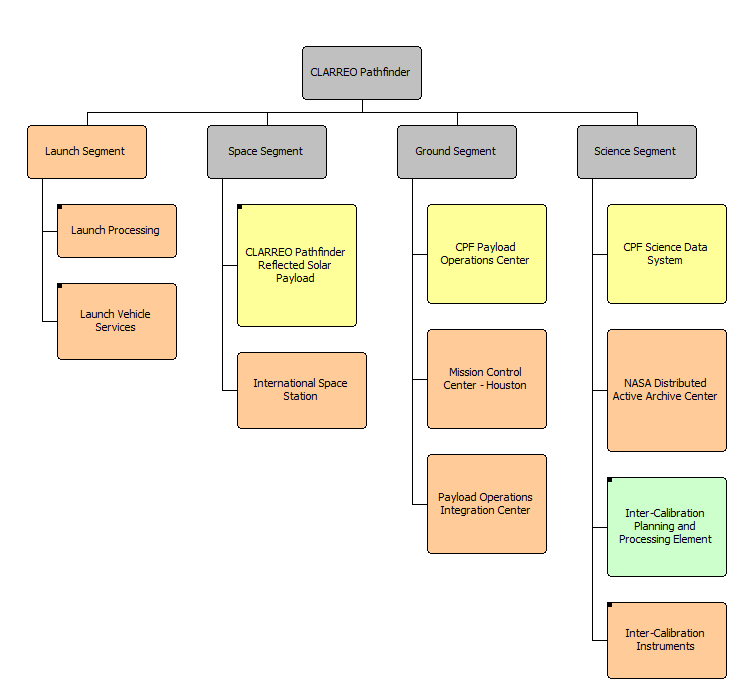
\includegraphics[keepaspectratio,width=5.75in,height=0.75\textheight]{20180416_cpf_architecture_l1-3.png}
\caption{\gls{CPF} System Architecture}
\label{cpf_arc}
\end{figure}

\section{Segment Definition }
\label{segmentdefinition}

\subsection{Space Segment }
\label{spacesegment}

The Space Segment is that portion of the architecture that flies in space and maintains the communication links between space and ground. It comprises the \gls{CPRSP} and the \gls{ISS}. The \gls{CPRSP} makes radiometric observations and transmits that information to the \gls{CPOC} via its attachment to the \gls{ISS}. The \gls{ISS} comprises the orbiting Space Station, all of its crew, visiting vehicles, attached non-\gls{CLARREO} Pathfinder payloads, and associated communications systems.

\subsection{Science Segment }
\label{sciencesegment}

The Science Segment includes all of the systems and facilities required to process, analyze (including calibration and validation of data), archive, and distribute the \gls{CPF} science data and data products. The Science Segment consists of four elements: the \gls{CSDS} at \gls{LASP}, a NASA \gls{DAAC}, the \gls{ICPP} element at \gls{LaRC}, and the Inter-Calibration Instruments. The Inter-Calibration Instruments are those specified by the On-Orbit Reference Inter-Calibration science objective. The NASA \gls{DAAC} will make the data products listed in the Standard Science Data Products table publicly available in accordance with NASA Earth Science Data and Information Policy with no period of exclusive access.

\subsection{Ground Segment }
\label{groundsegment}

The Ground Segment is the portion of the ground-based architecture that does not generate science products, and its primary role is to provide the monitoring, command, and control of the \gls{CPRSP}. It also processes and forwards the data received from the Space Segment to the Science Segment. It comprises the \gls{CPOC} at \gls{LASP}, \gls{MCC-H} at \gls{JSC}, and the \gls{POIC} at \gls{MSFC}.

\subsection{Launch Segment }
\label{launchsegment}

The Launch Segment is responsible for preparing the \gls{CPRSP} for flight and delivering it to the \gls{ISS}. The Launch Processing portion of the architecture prepares the \gls{CPRSP}, having completed final integration at \gls{KSC}, to function as an \gls{ISS} external payload. Launch Vehicle Services is the portion of the architecture responsible for transporting the \gls{CPRSP} from the Earth to the International Space Station. At this time, the identity of the Launch Vehicle Services provider and their associated requirements are not yet determined.

\chapter{Requirements  }
\label{sec_req}

\renewcommand\labelitemi{}

This section contains technical requirements, which define either what \gls{CPF} must do or a quality that the \gls{CPF} must have. Science Requirements trace directly to PLRA Baseline Science Requirements and specify performance of the overall \gls{CPF} mission. Mission Requirements allocate the \gls{SMRD} Science Requirements and PLRA Mission and Flight Element Performance Requirements to the Project-managed elements. The \gls{SMRD} groups Mission Requirements by segment.

The \gls{SMRD} distinguishes among requirements, goals, and statements of facts as follows:

\begin{itemize}
\item{} Shall: Used to indicate a binding requirement that will be verified

\item{} Should\slash May: Used to indicate a desired goal

\item{} Will: Used to indicate a statement of fact that the government will complete

\end{itemize}

The \gls{SMRD} allocates all Mission Requirements containing a ``shall'' to \gls{LASP}-managed elements. Goals are non-binding, while statements of fact are binding in that an expectation of certainty is established. Goals are included to guide trade studies and will be addressed at design reviews and technical interchange meetings. Values in this document listed as TBD or TBR are pending confirmation.

\section{Science Requirements}
\label{sciencerequirements}

\textbf{[CPF.20004]} Spectrally Resolved Earth Reflectance

The \gls{CLARREO} Pathfinder shall acquire on-orbit \gls{SI}-traceable spectrally resolved Earth reflectances referenced to spectral solar irradiance with average uncertainty <= 0.3\% (k=1) for the 350 - 2300 nm wavelength range.

\begin{itemize}
\item{} Rationale: \emph{To demonstrate on-orbit accuracy required for establishing climate change record.}

\item{} Parent Requirements: PLRA.10001

\item{} Verification Method: Inspection

\item{} Verification Description: The Project will inspect the closure artifacts of this requirement's children.

\item{} Success Criteria: The verification will be successful when all child requirements are closed.

\end{itemize}

\textbf{[CPF.20005]} Broadband Earth Reflectance

The \gls{CLARREO} Pathfinder shall acquire on-orbit \gls{SI}-traceable broadband reflectance (350 - 2300 nm) of Earth scenes with uncertainty <= 0.3\% (k=1).

\begin{itemize}
\item{} Rationale: \emph{To demonstrate on-orbit accuracy required for establishing climate change record}

\item{} Parent Requirements: PLRA.10006

\item{} Verification Method: Inspection

\item{} Verification Description: The Project will inspect the closure artifacts of this requirement's children.

\item{} Success Criteria: The verification will be successful when all child requirements are closed.

\end{itemize}

\textbf{[CPF.20050]} Inter-Calibration Samples

The \gls{CLARREO} Pathfinder shall \gls{collect} inter-calibration sampling with \gls{CERES} or \gls{RBI} and \gls{VIIRS} sufficient to limit uncertainty contribution within 1 year of operations as specified in requirements \gls{CPF}.20004 and \gls{CPF}.20005.

\begin{itemize}
\item{} Rationale: \emph{This specifies the need to perform inter-calibration with sufficient sampling to achieve the science requirements within a one year time frame. Inter-Calibration sampling refers to acquiring measurements of the surface radiance that coincides with the ground track of where CERES or RBI and VIIRS acquired their data from the Earth's surface.}

\item{} Parent Requirements: PLRA.10011

\item{} Verification Method: Inspection

\item{} Verification Description: The Project will inspect the closure artifacts of this requirement's children.

\item{} Success Criteria: The verification will be successful when all child requirements are closed.

\end{itemize}

\section{Mission Requirements}
\label{missionrequirements}

\subsection{Space Segment Requirements}
\label{spacesegmentrequirements}

\textbf{[RS.21000]} Wavelength

The \gls{CPRSP} shall \gls{measure} over the wavelength range of 350--2300 nm.

\begin{itemize}
\item{} Rationale: \emph{Values cover the range needed to observe changes in clouds, cloud phase, water vapor, aerosol, and land surface features. The upper limit is chosen due to loss of signal from reduced solar irradiance and strong water vapor and carbon dioxide absorption at longer wavelengths. The wavelength limits are chosen to provide sufficient spectral range for accurate intercalibration of the CERES broadband shortwave channels. Reference: Wu et al., 2015.}

\item{} Parent Requirements: PLRA.10030

\item{} Verification Method: Test

\item{} Verification Description: \gls{LASP} will \gls{test} the instrument by generating optical signals to stimulate every channel across the wavelength range.

\item{} Success Criteria: The verification will be successful when the \gls{CPRSP} responds to each channel over the range of 350--2300 nm.

\end{itemize}

\textbf{[RS.21004]} Spectrally Resolved Earth Reflectance

The \gls{CPRSP} shall acquire on-orbit \gls{SI}-traceable spectrally resolved Earth reflectances referenced to spectral solar irradiance with average uncertainty <= 0.3\% (k=1) for the 350 - 2300 nm wavelength range.

\begin{itemize}
\item{} Rationale: \emph{To demonstrate on-orbit accuracy required for establishing climate change record.}

\item{} Parent Requirements: \gls{CPF}.20004

\item{} Verification Method: Analysis

\item{} Verification Description: \gls{LASP} will analyze an uncertainty budget of the spectrally resolved reflectance.

\item{} Success Criteria: The verification will be successful when the error budget shows that the radiometric uncertainty is less than or uequal to 0.3\% at k=1.

\end{itemize}

\textbf{[RS.21005]} Broadband Earth Reflectance

The \gls{CPRSP} shall acquire on-orbit \gls{SI}-traceable broadband reflectance (350 - 2300 nm) of Earth scenes with uncertainty <= 0.3\% (k=1).

\begin{itemize}
\item{} Rationale: \emph{To demonstrate on-orbit accuracy required for establishing climate change record}

\item{} Parent Requirements: \gls{CPF}.20005

\item{} Verification Method: Analysis

\item{} Verification Description: \gls{LASP} will analyze an uncertainty budget of the broadband reflectance.

\item{} Success Criteria: The verification will be successful when the error budget shows that the radiometric uncertainty is less than or uequal to 0.3\% at k=1.

\end{itemize}

\textbf{[RS.21010]} Pointing Accuracy for Instrument Calibration

The \gls{CPRSP} shall have the ability to perform \gls{point}ing operations viewing Sun and Moon with sufficient accuracy to achieve uncertainty requirements \gls{RS}.21004 and \gls{RS}.21005.

\begin{itemize}
\item{} Rationale: \emph{The pointing requirement is driven by the along slit (flat field scan) of the sun and moon to consistently look at the same feature throughout the calibration.}

\item{} Parent Requirements: PLRA.10040, PLRA.10001

\item{} Verification Method: Analysis

\item{} Verification Description: \gls{LASP} will analyze the contribution of \gls{measure}d \gls{CPRSP} \gls{point}ing errors when viewing the Sun and Moon.

\item{} Success Criteria: The verification will be successful when the contribution of \gls{point}ing errors does not exceed the budget allocation associated with \gls{RS}.21004 and \gls{RS}.21005.

\end{itemize}

\textbf{[RS.21011]} Angular Matching for Inter-Calibration

The \gls{CPRSP} shall perform Inter-Calibration sampling by directing the \gls{HySICS} Instrument boresight to within 0.7 degree (k=1) of a time-varying direction that is determined by the line of sight from the Inter-Calibration Instrument (at some instant of time consistent with the temporal matching requirement) to the \gls{HySICS} Instrument.

\begin{itemize}
\item{} Rationale: \emph{To limit inter-calibration noise due to differences in viewing-zenith angles in HySICS and Inter-Calibration Instrument measurements. Wielicki et al., IGARSS 2008, specifies that at a point on Earth's surface within the Inter-Calibration Instrument's field of view, the viewing-zenith angles to that instrument and to HySICS should not differ by more than 1 degree. Measurements at the HySICS boresight meet this constraint when the boresight is aimed within 0.7 degrees of the time-varying line of sight. Reference CPF-SER-008.}

\item{} Parent Requirements: \gls{CPF}.20050, PLRA.10011, PLRA.10045

\item{} Verification Method: Analysis

\item{} Verification Description: \gls{LASP} will analyze the \gls{CPRSP}'s ability to track the lines of sight representative of a set of inter-calibration event geometries by programming the lines of sight and commanding the \gls{CPRSP} to track them.

\item{} Success Criteria: The verification will be successful when the error between the Inter-Calibration Instrument line of sight and the \gls{HySICS} Instrument boresight is less than 0.7 degrees (k=1) throughout the inter-calibration event.

\end{itemize}

\textbf{[RS.21012]} Temporal Matching for Inter-Calibration

The \gls{CPRSP} shall perform inter-calibration operations viewing Earth within 10 minutes of \gls{LEO} Inter-Calibration Instruments (CERES\slash RBI and VIIRS) data acquisition events.

\begin{itemize}
\item{} Rationale: \emph{For limiting inter-calibration noise due to time difference over viewed scene. Reference: Wielicki et al., IGARSS 2008.}

\item{} Parent Requirements: \gls{CPF}.20050, PLRA.10045

\item{} Verification Method: Analysis

\item{} Verification Description: \gls{LASP} will perform \gls{analysis} to show that the \gls{CPRSP} can execute an inter-calibration event. \gls{LaRC} will have to do the planning, but \gls{LASP} will have to perform \gls{analysis} showing the instrument can meet the requirement.

\item{} Success Criteria: The verification will be successful when the \gls{analysis} shows that the \gls{CPRSP} can execute the inter-calibration within 10 minutes of \gls{CERES}, \gls{RBI}, and \gls{VIIRS}.

\end{itemize}

\textbf{[RS.21015]} Spectral Sampling

The \gls{CPRSP} shall \gls{sample} at a spectral precision of 3 nm or finer, equivalent to a 6 nm full width half maximum Gaussian bandwidth.

\begin{itemize}
\item{} Rationale: \emph{Spectral sampling required to ensure < 0.2\% error from spectral resampling for inter-calibrating imager bands (VIIRS). Reference: Wu et al., 2015.}

\item{} Parent Requirements: PLRA.10011, PLRA.10035, PLRA.10001

\item{} Verification Method: Test

\item{} Verification Description: \gls{LASP} will \gls{test} the \gls{CPRSP} using multiple sources at varying wavelengths to ensure it can distinguish between the sources.

\item{} Success Criteria: The verification will be successful when the \gls{CPRSP} can distinguish between sources separated by 3 nm across the entire spectral range.

\end{itemize}

\textbf{[RS.21020]} Single Spectrum Precision for Inter-Calibration

The \gls{CPRSP} shall have a single spectrum precision of <= 3\% (k=1) relative to reflectance of 0.3 at solar zenith angle = 75 degrees. (This precision is at the scale of a single instantaneous 0.5 km field of view.)

\begin{itemize}
\item{} Rationale: \emph{The noise specification is set to enable clear versus cloudy screening and lunar calibration measurements.}

\item{} Parent Requirements: \gls{CPF}.20050, PLRA.10001

\item{} Verification Method: Test

\item{} Verification Description: \gls{LASP} will \gls{test} the precision of a \gls{CPRSP} single spectrum \gls{measure}ment relative to a \gls{test} signal with a reflectance of 0.3 at a solar zenith angle of 75 degrees.

\item{} Success Criteria: The verification will be successful when \gls{LASP} conducts a \gls{test} that proves that the \gls{CPRSP} single spectrum \gls{measure}ment, relative to \gls{test} signal with a reflectance of 0.3 at a solar zenith angle of 75 degrees, has a precision of 3\% (k=1) or better.

\end{itemize}

\textbf{[RS.21025]} Along-track \gls{FOV}

The \gls{CPRSP} shall \gls{measure} \gls{RS} radiation continuously along-track with a field of view less than or equal to 0.5 km at nadir.

\begin{itemize}
\item{} Rationale: \emph{This requirement is driven by the uncertainty budget for inter-calibration to limit noise from spatial data mapping, and the emphasis is gapless coverage along track. The actual instrument angular FOV, pixel size, and array geometry can be derived from this as well as the ISS altitude.}

\item{} Parent Requirements: PLRA.10011

\item{} Verification Method: Inspection

\item{} Verification Description: \gls{LASP} will inspect the \gls{CPRSP} design to determine the \gls{FOV} at \gls{ISS} altitude.

\item{} Success Criteria: The verification will be successful when the along-track field of view of the \gls{CPRSP} is less than or equal to 0.5 km.

\end{itemize}

\textbf{[RS.21030]} Along-track Ground Sampling Distance

The \gls{CPRSP} shall \gls{measure} \gls{RS} radiation continuously along-track with a ground-sampling distance less than or equal to 0.5 km at nadir.

\begin{itemize}
\item{} Rationale: \emph{The instrument enables the CLARREO continuous spatial sampling and matching required for inter-calibration, and the emphasis is along-track resolution. The actual instrument sampling rate, frame overlap, angular FOV, pixel size, and array geometry can be derived from this as well as the ISS altitude.}

\item{} Parent Requirements: PLRA.10011

\item{} Verification Method: Analysis

\item{} Verification Description: \gls{LASP} will analyze the \gls{CPRSP} sampling rate at \gls{ISS} altitude to determine the distance between resolved pixels.

\item{} Success Criteria: The verification will be successful when the distance between two pixels is 0.5 km or less.

\end{itemize}

\textbf{[RS.21031]} Cross-track Ground Sampling Distance

The \gls{CPRSP} shall \gls{measure} \gls{RS} radiation continuously cross-track with a ground-sampling distance less than or equal to 0.5 km at nadir.

\begin{itemize}
\item{} Rationale: \emph{The instrument enables the CLARREO continuous spatial sampling and matching required for inter-calibration. The actual instrument sampling rate, frame overlap, angular FOV, pixel size, and array geometry can be derived from this as well as the ISS altitude.}

\item{} Parent Requirements: PLRA.10011

\item{} Verification Method: Inspection

\item{} Verification Description: \gls{LASP} will inspect the \gls{CPRSP} design to show that when the pixels are averaged in the downlink that there will be sufficient surface resolution for inter-calibration in the cross track direction at nadir at \gls{ISS} altitude.

\item{} Success Criteria: The verification will be successful when the \gls{inspection} shows the \gls{CPRSP} can resolve two targets separated in the cross-track direction by an angle equivalent to 0.5 km.

\end{itemize}

\textbf{[RS.21035]} Instrument Sensitivity to Polarization

The \gls{CPRSP} shall \gls{measure} the \gls{RS} radiation in the reflected solar spectra as a reference calibration to relevant climate sensors with polarization sensitivity less than 1\% (k=1) in wavelength range from 350 - 1800 nm and less than 2\% (k=1) from 1800 - 2300nm.

\begin{itemize}
\item{} Rationale: \emph{This requirement ensures that the uncertainty contribution form instrument sensitivity to polarization is limited. Simulations were carried out to determine the distribution of spectrally dependent polarization using global PARASOL multi-angle, multi-spectral polarization measurements. The data were used to simulate the polarization distributions across a full range of scene conditions and climate regions that CLARREO would see for its nadir reflectance spectra, as well as for the scattering angles that it would use to provide Reference Intercalibration to CERES or RBI and VIIRS. Reference: Lukashin et al., 2013.}

\item{} Parent Requirements: PLRA.10011, PLRA.10001

\item{} Verification Method: Test

\item{} Verification Description: \gls{LASP} will \gls{test} the difference in response of the \gls{CPRSP} to a polarized signal versus a non-polarized signal.

\item{} Success Criteria: The verification will be successful when the difference in response in the polarized signal versus the non-polarized signal is less than 1\% (k=1) in wavelength range from 350 - 1800 nm and less than 2\% (k=1) from 1800 - 2300nm.

\end{itemize}

\textbf{[RS.21040]} Prime Mission Operations Period

The \gls{CPRSP} shall operate over a prime mission operation period of 1 year following commissioning activities.

\begin{itemize}
\item{} Rationale: \emph{CLARREO Pathfinder is a directed mission with 1 year of operations.}

\item{} Parent Requirements: PLRA.10115

\item{} Verification Method: Analysis

\item{} Verification Description: \gls{LASP} will analyze the expected \gls{CPRSP} operational lifetime.

\item{} Success Criteria: The verification will be successful when the \gls{analysis} shows the expected operational lifetime is greater than or equal to 1 year.

\end{itemize}

\textbf{[RS.21041]} On-Orbit Commissioning Period

The \gls{CPRSP} shall complete commissioning activities within 60 days of installation to the \gls{ISS}.

\begin{itemize}
\item{} Rationale: \emph{Two months provide sufficient time for functionality tests of the CPRSP.}

\item{} Parent Requirements: PLRA.10120

\item{} Verification Method: Analysis

\item{} Verification Description: \gls{LASP} will analyze the expected duration of all required \gls{CPRSP} commissioning activities.

\item{} Success Criteria: The verification will be successful when the \gls{analysis} shows the \gls{CPRSP} commissioning activities can be completed within 60 days.

\end{itemize}

\textbf{[RS.21045]} Decommissioning

The \gls{CPRSP} shall be capable of completing decommissioning activities within three months following the end of the science mission.

\begin{itemize}
\item{} Rationale: \emph{The three-month measure establishes a time limit for the CPRSP to be configured for disposal.}

\item{} Parent Requirements: PLRA.10122

\item{} Verification Method: Analysis

\item{} Verification Description: \gls{LASP} will analyze the expected duration of all required \gls{CPRSP} decommissioning activities.

\item{} Success Criteria: The verification will be successful when the \gls{analysis} shows the \gls{CPRSP} decommissioning activities can be completed within three months.

\end{itemize}

\textbf{[RS.21055]} Inter-Calibration Swath Width

The \gls{CPRSP} shall be capable of aiming the instrument boresight to match the full \gls{CERES}, \gls{RBI}, and \gls{VIIRS} instrument swath width (plus or minus 55°) when not obscured by \gls{ISS} structure.

\begin{itemize}
\item{} Rationale: \emph{This enables sufficient inter-calibration sampling with instruments flying in JPSS-like orbits. The reference is to the ISS body axes instead of the ISS ground track, due to the contribution of ISS attitude excursions to ground-referenced lines of sight. Reference: MCR Inter-Calibration Approach presentation (Section 10.0).}

\item{} Parent Requirements: PLRA.10011, PLRA.10001

\item{} Verification Method: Analysis

\item{} Verification Description: \gls{LASP} will analyze the FOR of the \gls{CPRSP} \gls{point}ing capability, with typical \gls{ISS} attitude excursions.

\item{} Success Criteria: The verification will be successful when the \gls{analysis} shows that the FOR can accommodate the \gls{CERES}, \gls{RBI}, and \gls{VIIRS} instrument swath width when not obscured by \gls{ISS} structure.

\end{itemize}

\textbf{[RS.21060]} Geolocation of Earth-View Data

The \gls{CPRSP} shall have sufficient \gls{point}ing knowledge such that the \gls{CSDS} can determine the Earth viewing pixel geolocation to within 250 m (k=1) nadir equivalent.

\begin{itemize}
\item{} Rationale: \emph{This enables the CSDS to generate geolocated data at a precision of 250 m, which is one half of a single pixel's footprint; maintaining this performance ensures that the target point falls within the pixel's actual footprint. This limits the inter-calibration noise due to spatial difference over the viewed scene. Reference: Wielicki et al., IGARSS 2008}

\item{} Parent Requirements: PLRA.10045

\item{} Verification Method: Analysis

\item{} Verification Description: \gls{LASP} will verify by \gls{analysis}.

\item{} Success Criteria: The verification will be successful when the \gls{analysis} shows that the \gls{CPRSP} has sufficient \gls{point}ing knowledge such that the \gls{CSDS} can determine pixel geolocation within 250 m.

\end{itemize}

\textbf{[RS.21110]} Swath Width

The \gls{CPRSP} shall \gls{measure} \gls{RS} radiation with a cross-track width greater than or equal to 70 km when centered at nadir.

\begin{itemize}
\item{} Rationale: \emph{The specific spatial extent is required to ensure sufficient inter-calibration spatial sampling with relevant instruments. Reference: science study report: SS-2002f-01; Wielicki et al., IGARSS 2008.}

\item{} Parent Requirements: PLRA.10011

\item{} Verification Method: Analysis

\item{} Verification Description: \gls{LASP} will document the \gls{CPRSP} design.

\item{} Success Criteria: The verification will be successful when the \gls{inspection} shows that the \gls{CPRSP}'s nadir field-of-view footprint is greater than or equal to 70 km.

\end{itemize}

\textbf{[RS.21150]} Inter-Calibration Operations

The \gls{CPRSP} shall be capable of performing 1 Inter-Calibration operation per orbit. An Inter-Calibration operation is defined as one of the following:

\begin{itemize}
\item{} - Measurement of spectral reflectance over entire lunar disk

\item{} - Inter-Calibration of space-borne instruments in low Earth orbit (LEO)

\item{} - Inter-Calibration of space-borne instruments in geostationary Earth orbit (GEO)

\item{} Rationale: \emph{To ensure that there will be adequate pointing capability in the HPS to perform all of the Inter-Calibration operations during the mission life. The intent of this requirement is that if there is an opportunity for an Inter-Calibration measurement during an orbit, the CPRSP should be able to acquire the data. This requirement in not intended to drive the CPRSP to add additional hardware.\\
Science Rationale: There will be approximately 1300 inter-calibration opportunities with JPSS instruments (CERES or RBI and VIIRS) per year. The CPRSP needs to be capable of taking data for every opportunity.}

\item{} Parent Requirements: \gls{CPF}.20050, PLRA.10011, PLRA.10001

\item{} Verification Method: Analysis

\item{} Verification Description: \gls{LASP} will analyze the \gls{point}ing system of the \gls{CPRSP} to make sure that the design supports the number of Inter-Calibration operations.

\item{} Success Criteria: The verification will be successful when the \gls{analysis} shows that the \gls{CPRSP} can perform at least one representative inter-calibration \gls{point}ing event per orbit over the one year primary mission without exceeding the designed system's expected service life.

\end{itemize}

\textbf{[RS.22000]} Compliance with Launch Vehicle Requirements

The \gls{CPRSP} shall satisfy the launch vehicle requirements.

\begin{itemize}
\item{} Rationale: \emph{Compliance with LV requirements maximizes probability of successful integration with the LV and mission success. (SSP-50833)}

\item{} Parent Requirements: PLRA.10125

\item{} Verification Method: Inspection

\item{} Verification Description: \gls{LASP} will inspect all Launch Vehicle Services-levied requirements to ensure compliance.

\item{} Success Criteria: The verification will be successful when the Launch Vehicle Services-levied requirements have been successfully verified.

\end{itemize}

\textbf{[RS.22005]} Compliance with \gls{ISS} Requirements

The \gls{CPRSP} shall satisfy \gls{ISS} requirements.

\begin{itemize}
\item{} Rationale: \emph{Compliance with ISS requirements maximizes probability of successful integration with the ISS and mission success.}

\item{} Parent Requirements: PLRA.10025, PLRA.10020

\item{} Verification Method: Inspection

\item{} Verification Description: \gls{LASP} will inspect all \gls{ISS}-levied requirements to ensure compliance.

\item{} Success Criteria: The verification will be successful when the \gls{ISS}-levied requirements have been successfully verified.

\end{itemize}

\textbf{[RS.22010]} Compliance with Payload Interface Agreement Resource Allocations

The \gls{CPRSP} shall comply with the resource allocations documented within the \gls{CPF} to \gls{ISS} \gls{PIA}.

\begin{itemize}
\item{} Rationale: \emph{The PIA PIP-16--039 states a more restrictive resource allocation than the ISS Interface Requirements Baseline. The CPRSP is expected to meet the resources specified in the PIA.}

\item{} Parent Requirements: PLRA.10020

\item{} Verification Method: Inspection

\item{} Verification Description: \gls{LASP} will inspect the artifacts of relevant lower level verifications and compare them against all of the resource allocations specified by the \gls{PIA}.

\item{} Success Criteria: The verification will be successful when the artifacts of the relevant lower level verifications show compliance with all of the resource allocations specified by the \gls{PIA}.

\end{itemize}

\textbf{[RS.22025]} Measurements and Data Routing

The \gls{CPRSP} shall send science \gls{measure}ments and data to the \gls{CPOC}.

\begin{itemize}
\item{} Rationale: \emph{The CPRSP will send raw (unprocessed) science measurements, health and status data, contamination, disturbance, and ancillary data via the ISS. The POIC will forward all data to the CPOC.}

\item{} Parent Requirements: PLRA.10001

\item{} Verification Method: Demonstration

\item{} Verification Description: \gls{LASP} will demonstrate that the \gls{CPRSP} can properly send science \gls{measure}ments and data back to the \gls{CPOC}.

\item{} Success Criteria: The verification will be successful when the \gls{CPRSP} has completed the \gls{demonstration}.

\end{itemize}

\textbf{[RS.22035]} Response to Ground Commands

The \gls{CPRSP} shall have the capability to accept ground commands.

\begin{itemize}
\item{} Rationale: \emph{The CPRSP operates using time-tagged sequences or real-time commands uploaded from the CPOC. Reference: CPF-02--009, Section 6.3 (29AUG2017)}

\item{} Parent Requirements: PLRA.10011, PLRA.10001

\item{} Verification Method: Demonstration

\item{} Verification Description: \gls{LASP} will demonstrate that the \gls{CPRSP} can receive commands from the \gls{CPOC} through the \gls{ELC} simulator at \gls{KSC}.

\item{} Success Criteria: The verification will be successful when the \gls{CPRSP} has completed the \gls{demonstration}.

\end{itemize}

\textbf{[RS.22040]} On-orbit Reprogramming

The \gls{CPRSP} shall have the capability of being reprogrammed while on orbit.

\begin{itemize}
\item{} Rationale: \emph{On-orbit reprogramming allows flight controllers and command controllers to update the CPRSP's behavior to accommodate unexpected demands of the operating environment.}

\item{} Parent Requirements: PLRA.10011, PLRA.10006, PLRA.10001

\item{} Verification Method: Demonstration

\item{} Verification Description: \gls{LASP} will demonstrate the \gls{CPRSP} reprogrammability capability by transmitting a \gls{CPRSP} software update at the \gls{CPOC} and identifying the software load of the \gls{CPRSP} at the \gls{ELC} simulator.

\item{} Success Criteria: The verification will be successful when the \gls{CPRSP} software load matches the update transmitted at the \gls{CPOC}.

\end{itemize}

\subsection{Science Segment Requirements}
\label{sciencesegmentrequirements}

\subsubsection{Science Segment Requirements - LASP}
\label{sciencesegmentrequirements-lasp}

\textbf{[SCI.24000]} Data Product Delivery

The \gls{CSDS} shall deliver all Level 0 and Level 1B data products to the NASA \gls{DAAC} within the timelines specified for each data product in the Standard Science Data Products table.

\begin{itemize}
\item{} Rationale: \emph{References: 152-TP-003--003 and GSFC 423-SPEC-001.}

\item{} Parent Requirements: PLRA.10145, PLRA.10146

\item{} Verification Method: Test

\item{} Verification Description: \gls{LASP} will \gls{test} that the \gls{CSDS} can deliver Level 0 and Level 1B data products to the NASA \gls{DAAC}.

\item{} Success Criteria: The verification will be successful when the \gls{DAAC} reports receipt of Level 0 and Level 1B data.

\end{itemize}


\begin{table}[htbp]
\begin{minipage}{\linewidth}
\setlength{\tymax}{0.5\linewidth}
\centering
\small
\caption{Standard Science Data Products}
\label{tbl_std_sci_data_prod}
\begin{threeparttable}
\begin{tabulary}{\textwidth}{|+p{1.0in}|^p{3.0in}|^p{0.75in}|^p{0.75in}|} \hline
\rowstyle{\bfseries}%
\rowstyle{\bfseries}%
 Data Product & Description                                                         & First Data Delivery after IOC & Maximum data latency after first release\tnote{1} \\
\hline
 Level 0   & Reconstructed, unprocessed instrument and payload data at full resolution, with any and all communications artifacts (e.g., synchronization frames, communications headers, duplicate data) removed.           & 4 months       & 48 hours         \\
 Level 1B  & Calibrated and geolocated observations at full resolution, annotated with ancillary information such as radiometric and geometric calibration coefficients and georeferencing parameters (e.g., platform ephemeris).       & 8 months       & 1 month         \\
 Level 4   & Time\slash angle\slash space matched inter--calibration data for reference (CPF) and target sensors (CERES or RBI and VIIRS), scene information from target sensors (CERES or RBI and VIIRS), modeled parameters for estimated polarization and radiometric corrections. & 10 months      & 6 months         \\
\hline
\end{tabulary}
\begin{tablenotes}
\item[1] Data latency is defined as the elapsed time from the downlink to the availability of processed data products to the public.
\end{tablenotes}
\end{threeparttable}
\end{minipage}
\end{table}


\textbf{[SCI.24015]} Public Release of Data

The \gls{CSDS} shall make the Level 0 and Level 1B data listed in the Standard Science Data Products table, along with the scientific source code for algorithm software, coefficients, and ancillary data used to generate these products publicly available conforming to the NASA Earth Science Data and Information Policy (http:\slash \slash science.nasa.gov\slash earth-science\slash earth-science-data\slash data-information-policy\slash ).

\begin{itemize}
\item{} Rationale: \emph{References: 152-TP-003--003 and GSFC 423-SPEC-001.}

\item{} Parent Requirements: PLRA.10145, PLRA.10146

\item{} Verification Method: Test

\item{} Verification Description: \gls{LASP} will \gls{test} that the \gls{CSDS} can deliver the Level 0 and Level 1B data, scientific source code for algorithm software, coefficients, and ancillary data used to generate these data products to the NASA \gls{DAAC}.

\item{} Success Criteria: The verification will be successful when the \gls{DAAC} reports receipt of the Level 0 data, Level 1B data, science source code, coefficients, and ancillary data.

\end{itemize}

\textbf{[SCI.24017]} Science Data Product Formats

The \gls{CSDS} shall format all Level 1B data products to conform to the HDF5 standard.

\begin{itemize}
\item{} Rationale: \emph{This enables compliance with the NASA Earth Science Data and Information Policy.}

\item{} Parent Requirements: PLRA.10205

\item{} Verification Method: Inspection

\item{} Verification Description: \gls{LASP} will inspect the Level 1B data product format.

\item{} Success Criteria: The verification will be successful when the \gls{inspection} shows that the Level 1B data products conform to the HDF5 standard.

\end{itemize}

\textbf{[SCI.24018]} Long Term Knowledge Preservation

The \gls{CSDS} shall transfer to the NASA \gls{DAAC} all the information and documentation required for long-term preservation of knowledge about the Level 0 and Level 1B data products as defined in the NASA Earth Science Data Preservation Content Specification document published at http:\slash \slash earthdata.nasa.gov\slash about-eosdis\slash requirements.

\begin{itemize}
\item{} Rationale: \emph{This enables compliance with the NASA Earth Science Data Preservation Content Specification document published at http:\slash \slash earthdata.nasa.gov\slash about-eosdis\slash requirements.}

\item{} Parent Requirements: PLRA.10220

\item{} Verification Method: Test

\item{} Verification Description: \gls{LASP} will \gls{test} that the \gls{CSDS} can deliver the required set of information and documentation to the NASA \gls{DAAC}.

\item{} Success Criteria: The verification will be successful when the \gls{DAAC} reports receipt of the information and documentation.

\end{itemize}

\textbf{[SCI.24020]} Mission Lifetime - \gls{LASP}

The \gls{CSDS} shall be designed to support 60 days of commissioning, a prime mission operation period of 1 year, and 1 year of science post processing following the prime mission operation period.

\begin{itemize}
\item{} Rationale: \emph{Science Segment operations and hardware must be designed to support operations throughout the mission duration.}

\item{} Parent Requirements: PLRA.10150

\item{} Verification Method: Inspection

\item{} Verification Description: \gls{LASP} will inspect \gls{LASP} \gls{CSDS} operational planning documentation on personnel, schedule, and funding.

\item{} Success Criteria: The verification will be successful when the \gls{LASP} \gls{CSDS} operational planning documentation identifies the commitment of key personnel, sufficient funding, and facilities supporting \gls{CPF} science for a duration of at least two years following commissioning activities.

\end{itemize}

\textbf{[SCI.24031]} Post Processing Geolocation for Earth-View Data

The \gls{CSDS} shall determine the geolocation of the Earth viewing pixels within 250 m (k=1) nadir equivalent.

\begin{itemize}
\item{} Rationale: \emph{The LASP CLARREO Science Data System (CSDS) shall determine the geolocation of the Earth viewing pixels within 250 m (k=1) nadir equivalent. Reference: Wielicki et al., IGARSS 2008}

\item{} Parent Requirements: PLRA.10045

\item{} Verification Method: Analysis

\item{} Verification Description: \gls{LASP} will analyze the \gls{CSDS}'s capability to geolocate the Earth viewing pixels.

\item{} Success Criteria: The verification will be successful when the \gls{analysis} shows the \gls{CSDS} can geolocate the Earth viewing pixels within 250 m (k=1).

\end{itemize}

\textbf{[SCI.24035]} Data Latency

The \gls{CSDS} shall deliver all required data to the NASA \gls{DAAC} within the timeframe specified in the Standard Science Data Products table.

\begin{itemize}
\item{} Rationale: \emph{The DAAC is the architectural element responsible for ingesting and archiving CPF data products, and the timeframe ensures efficient public dissemination.}

\item{} Parent Requirements: PLRA.10150

\item{} Verification Method: Inspection

\item{} Verification Description: \gls{LASP} will inspect their mission operations requirements for compliance with the data delivery timeline given in the table.

\item{} Success Criteria: The verification will be successful when \gls{LASP} shows data will be delivered according to Table 1.

\end{itemize}

\textbf{[SCI.24040]} \gls{ESDIS} Compliance

The \gls{CSDS} shall generate Level 0 and Level 1B data products whose metadata conform to ISO 19115 Geographic Information - Metadata standards and adhere to the Metadata Requirements --- Base Reference for NASA Earth Science Data Products document published at http:\slash \slash earthdata.nasa.gov\slash about-eosdis\slash requirements.

\begin{itemize}
\item{} Rationale: \emph{The NASA Earth Science Data and Information Policy is specified at http:\slash \slash science.nasa.gov\slash earth-science\slash earth-science-data\slash data-information-policy\slash . Items include Algorithm Theoretical Basis Documents and science algorithm source code.}

\item{} Parent Requirements: PLRA.10150, PLRA.10146, PLRA.10210

\item{} Verification Method: Test

\item{} Verification Description: \gls{LASP} will verify by \gls{test} that the \gls{CSDS} can deliver metadata conforming to ISO 19115 to the NASA \gls{DAAC}.

\item{} Success Criteria: The verification will be successful when the \gls{DAAC} reports receipt of the metadata.

\end{itemize}

\textbf{[SCI.24050]} Full Resolution Browse Products

The \gls{CSDS} shall deliver to the NASA \gls{DAAC} full-resolution browse products for all science data.

\begin{itemize}
\item{} Rationale: \emph{Full-resolution browse products enable users to search for specific scenes generated from CLARREO Pathfinder Reflected Solar Payload data. The specification of ``science data'' refers to data that is destined to the DAAC for science purposes, as opposed to data collected for engineering analysis.}

\item{} Parent Requirements: PLRA.10215

\item{} Verification Method: Demonstration

\item{} Verification Description: \gls{LASP} will demonstrate that the \gls{CSDS} can deliver browse products to the NASA \gls{DAAC}.

\item{} Success Criteria: The verification will be successful when the \gls{DAAC} reports the receipt of the browse products.

\end{itemize}

\subsubsection{Science Segment Requirements - LaRC}
\label{sciencesegmentrequirements-larc}

\textbf{[SCI.24100]} Data Product Delivery

The \gls{ICPP} will deliver all Level 4 data products to the NASA \gls{DAAC} within the timelines specified for first data delivery associated with each data product in the Standard Science Data Products table.

\begin{itemize}
\item{} Rationale: \emph{References: 152-TP-003--003 and GSFC 423-SPEC-001.}

\item{} Parent Requirements: PLRA.10145, PLRA.10146

\item{} Verification Method: Test

\item{} Verification Description: \gls{LaRC} will verify by \gls{test} that the \gls{ICPP} can deliver Level 4 data products to the NASA \gls{DAAC}.

\item{} Success Criteria: The verification will be successful when the \gls{DAAC} reports receipt of Level 4 data products.

\end{itemize}

\textbf{[SCI.24115]} Public Release of Data

The \gls{ICPP} will make the Level 4 data listed in the Standard Science Data Products table, along with the scientific source code for algorithm software, coefficients, and ancillary data used to generate these products publicly available conforming to the NASA Earth Science Data and Information Policy (http:\slash \slash science.nasa.gov\slash earth-science\slash earth-science-data\slash data-information-policy\slash ).

\begin{itemize}
\item{} Rationale: \emph{References: 152-TP-003--003 and GSFC 423-SPEC-001.}

\item{} Parent Requirements: PLRA.10145, PLRA.10146

\item{} Verification Method: Test

\item{} Verification Description: \gls{LaRC} will \gls{test} that the \gls{ICPP} can deliver the Level 4 data, scientific source code for algorithm software, and the coefficients and ancillary data used to generate these data products to the NASA \gls{DAAC}.

\item{} Success Criteria: The verification will be successful when the \gls{DAAC} reports receipt of the Level 4 data, science source code for algorithm software, coefficients, and ancillary data used to generate these products.

\end{itemize}

\textbf{[SCI.24117]} Science Data Product Formats

The \gls{ICPP} will format all Level 4 data products to conform to the HDF5 standard.

\begin{itemize}
\item{} Rationale: \emph{This enables compliance with the NASA Earth Science Data and Information Policy.}

\item{} Parent Requirements: PLRA.10205

\item{} Verification Method: Inspection

\item{} Verification Description: \gls{LaRC} will inspect the Level 4 data product format.

\item{} Success Criteria: The verification will be successful when \gls{inspection}s show that the Level 4 data products conform to the HDF5 standard.

\end{itemize}

\textbf{[SCI.24118]} Long Term Knowledge Preservation

The \gls{ICPP} will transfer to the NASA \gls{DAAC} all the information and documentation required for long-term preservation of knowledge about the Level 4 data products as defined in the NASA Earth Science Data Preservation Content Specification document published at http:\slash \slash earthdata.nasa.gov\slash about-eosdis\slash requirements.

\begin{itemize}
\item{} Rationale: \emph{This enables compliance with the NASA Earth Science Data and Information Policy.}

\item{} Parent Requirements: PLRA.10220

\item{} Verification Method: Test

\item{} Verification Description: \gls{LaRC} will \gls{test} that the \gls{ICPP} can deliver the required set of information and documentation to the NASA \gls{DAAC}.

\item{} Success Criteria: The verification will be successful when the \gls{DAAC} reports receipt of the information and documentation.

\end{itemize}

\textbf{[SCI.24120]} Mission Lifetime - \gls{LaRC}

The \gls{ICPP} will be designed to support 60 days of commissioning, a prime mission operation period of 1 year, and 1 year of science post processing following the prime mission operation period.

\begin{itemize}
\item{} Rationale: \emph{Science Segment operations and hardware must be designed to support operations throughout the mission duration.}

\item{} Parent Requirements: PLRA.10150

\item{} Verification Method: Inspection

\item{} Verification Description: \gls{LaRC} will inspect the \gls{LaRC} \gls{ICPP} operational planning documentation on personnel, schedule, and funding.

\item{} Success Criteria: The verification will be successful when \gls{LASP} \gls{ICPP} operational planning documentation identifies the commitment of key personnel, sufficient funding, and a facility dedicated to \gls{CPF} science for a duration of at least two years following commissioning activities.

\end{itemize}

\textbf{[SCI.24126]} Inter-Calibration Planning

The \gls{ICPP} will provide the inter-calibration planning data to the \gls{CPOC} according to the \gls{CPOC} interface control document.

\begin{itemize}
\item{} Rationale: \emph{The ICPP identifies and prioritizes the expected inter-calibration events and passes the list of prioritized inter-calibration targets to the CPOC. Reference: CPF-02--009, Section 6.2.1 (29AUG2017)}

\item{} Parent Requirements: PLRA.10150

\item{} Verification Method: Test

\item{} Verification Description: \gls{LaRC} will verify by \gls{test} that the \gls{ICPP} can deliver the inter-calibration planning data to the \gls{CPOC} according to the \gls{CPOC} interface control document

\item{} Success Criteria: The verification will be successful when the \gls{CPOC} reports receipt of inter-calibration planning data.

\end{itemize}

\textbf{[SCI.24130]} Inter-Calibrate Science Data

The \gls{ICPP} will inter-calibrate \gls{CLARREO} Pathfinder science data with \gls{VIIRS}.

\begin{itemize}
\item{} Rationale: \emph{The ICPP retrieves VIIRS Level 1B and Level 2 data from the LAADS at GSFC and applies inter-calibration algorithms to produce Level 4 data products. Reference: CPF-02--009, Section 10.4 (27AUG017)}

\item{} Parent Requirements: PLRA.10150

\item{} Verification Method: Analysis

\item{} Verification Description: \gls{LaRC} will perform the inter-calibration \gls{analysis} using a set of \gls{VIIRS} data products from the \gls{LAADS} \gls{DAAC} and a set of internally-generated \gls{CPF} Level 1B data.

\item{} Success Criteria: The verification will be successful when the \gls{analysis} shows the inter-calibration requirements have been met.

\end{itemize}

\textbf{[SCI.24131]} Inter-Calibrate Science Data

The \gls{ICPP} will inter-calibrate \gls{CLARREO} Pathfinder science data with \gls{CERES}\slash \gls{RBI}.

\begin{itemize}
\item{} Rationale: \emph{The ICPP retrieves CERES and RBI Level 2 data from the ASDC at LaRC and applies inter-calibration algorithms to produce Level 4 data products. Reference: CPF-02--009, Section 10.4 (27AUG017)}

\item{} Parent Requirements: PLRA.10150

\item{} Verification Method: Analysis

\item{} Verification Description: \gls{LaRC} will perform the inter-calibration \gls{analysis} using a set of \gls{CERES} and \gls{RBI} data products from the \gls{ASDC} \gls{DAAC} and a set of internally-generated \gls{CPF} Level 1B data.

\item{} Success Criteria: The verification will be successful when the \gls{analysis} shows the inter-calibration requirements have been met.

\end{itemize}

\textbf{[SCI.24140]} \gls{ESDIS} Compliance

The \gls{ICPP} will generate Level 4 data products whose metadata conform to ISO 19115 Geographic Information - Metadata standards and adhere to the Metadata Requirements --- Base Reference for NASA Earth Science Data Products document published at http:\slash \slash earthdata.nasa.gov\slash about-eosdis\slash requirements.

\begin{itemize}
\item{} Rationale: \emph{The NASA Earth Science Data and Information Policy is specified at http:\slash \slash science.nasa.gov\slash earth-science\slash earth-science-data\slash data-information-policy\slash . Items include Algorithm Theoretical Basis Documents and science algorithm source code.}

\item{} Parent Requirements: PLRA.10150, PLRA.10146, PLRA.10210

\item{} Verification Method: Test

\item{} Verification Description: \gls{LaRC} will \gls{test} that the \gls{ICPP} can deliver metadata conforming to ISO 19115 to the NASA \gls{DAAC}.

\item{} Success Criteria: The verification will be successful when the \gls{DAAC} reports receipt of the metadata.

\end{itemize}

\subsection{Ground Segment Requirements}
\label{groundsegmentrequirements}

\textbf{[GS.23000]} \gls{POIC} Interface

The \gls{CPOC} shall interface with the \gls{ISS} \gls{POIC} in accordance with the \gls{CPOC} to \gls{POIC} ICD (TBD).

\begin{itemize}
\item{} Rationale: \emph{Nominally, all CPRSP commands flow from the CPOC through the POIC, and all Raw TLM and Science data flow through the POIC to the CPOC. Reference: CPF-02--009, Section 5.3 (29AUG2017). The ISS Program will furnish a future document that will specify the CPOC to POIC interface.}

\item{} Parent Requirements: PLRA.10145, PLRA.10140

\item{} Verification Method: Test

\item{} Verification Description: \gls{LASP} will \gls{test} the \gls{CPOC} to \gls{POIC} interface.

\item{} Success Criteria: The verification will be successful when all of the \gls{CPOC} to \gls{POIC} interface requirements have been met.

\end{itemize}

\label{tbx_1}

\textbf{[GS.23005]} Generate Instrument Commanding

The \gls{CPOC} shall generate instrument commands and command loads for the execution of all \gls{CPRSP} functions on orbit.

\begin{itemize}
\item{} Rationale: \emph{The CPOC generates all of the commands sent to the CPRSP. Reference: CPF-02--009, Section 4.3.1 (29AUG2017)}

\item{} Parent Requirements: PLRA.10145, PLRA.10140

\item{} Verification Method: Demonstration

\item{} Verification Description: \gls{LASP} will demonstrate that the \gls{CPOC} can properly format \gls{CPRSP} commands.

\item{} Success Criteria: The verification will be successful when the \gls{CPOC} has shown that it can properly format commands for transmission to the \gls{CPRSP}.

\end{itemize}

\textbf{[GS.23010]} Transfer Command Information

The \gls{CPOC} shall transfer commands and command loads to the \gls{POIC} for upload to the \gls{ISS}.

\begin{itemize}
\item{} Rationale: \emph{The CPOC sends commands and any file uploads to the POIC for transfer to the Space Segment. Reference: CPF-02--009, Section 5.3 (29AUG2017)}

\item{} Parent Requirements: PLRA.10145, PLRA.10140

\item{} Verification Method: Demonstration

\item{} Verification Description: \gls{LASP} will demonstrate that the \gls{CPOC} can send \gls{CPRSP} commands to the \gls{POIC}.

\item{} Success Criteria: The verification will be successful when the \gls{POIC} receives commands and command loads from the \gls{CPOC}.

\end{itemize}

\textbf{[GS.23015]} Validate Commands and Command Loads

The \gls{CPOC} shall validate commands and command loads prior to sending them to the \gls{POIC} for uploading to the \gls{CPRSP}.

\begin{itemize}
\item{} Rationale: \emph{CPOC validation of commands and command loads ensure that they have the intended effect on the CPRSP and do not risk the health or safety of the CPRSP. Reference: CPF-02--009, Section 6.3 (29AUG2017)}

\item{} Parent Requirements: PLRA.10145, PLRA.10140

\item{} Verification Method: Test

\item{} Verification Description: \gls{LASP} will \gls{test} the \gls{CPRSP} command responses prior to transmission to the \gls{POIC}.

\item{} Success Criteria: The verification will be successful when \gls{test}ing shows that commands are validated before sending to the \gls{POIC}.

\end{itemize}

\textbf{[GS.23020]} Generate Instrument Software Loads

The \gls{CPOC} shall generate instrument software loads to support \gls{CPRSP} operations.

\begin{itemize}
\item{} Rationale: \emph{CPOC generation of instrument software loads enables the On-orbit reprogramming specified in RS.22040.}

\item{} Parent Requirements: PLRA.10145, PLRA.10140

\item{} Verification Method: Demonstration

\item{} Verification Description: \gls{LASP} will demonstrate that the Ground Segment can generate valid software that can be loaded onto the \gls{CPRSP}.

\item{} Success Criteria: The verification will be successful when the Ground Segment produces a valid software load.

\end{itemize}

\textbf{[GS.23030]} Health Maintenance of the Space Segment

The \gls{CPOC} shall monitor the health and safety of the \gls{CPRSP} and generate advisories of potentially unsafe conditions.

\begin{itemize}
\item{} Rationale: \emph{One of the primary functions of the CPOC is to employ state of health monitoring of the CPRSP on a daily basis. Reference: CPF-02--009, Section 6.4 (29AUG2017)}

\item{} Parent Requirements: PLRA.10145, PLRA.10140

\item{} Verification Method: Demonstration

\item{} Verification Description: \gls{LASP} will demonstrate that advisories will be generated for potentially unsafe \gls{CPRSP} conditions.

\item{} Success Criteria: The verification will be successful when the \gls{CPOC} generates the advisories.

\end{itemize}

\textbf{[GS.23035]} Science Event Measurement Planning

The \gls{CPOC} shall have the capability of planning \gls{CPRSP} flight operations.

\begin{itemize}
\item{} Rationale: \emph{The CPOC planning process uses information from various sources in order to generate the necessary command products for the CPRSP. Reference: CPF-02--009, Section 6.2 (29AUG2017)}

\item{} Parent Requirements: PLRA.10145, PLRA.10140

\item{} Verification Method: Demonstration

\item{} Verification Description: \gls{LASP} will demonstrate that the \gls{CPOC} can plan flight operations.

\item{} Success Criteria: The verification will be successful when the Ground Segment can generate a plan flight operations for all science events.

\end{itemize}

\textbf{[GS.23040]} Prime Mission Operational Lifetime

The \gls{CPOC} shall be designed to operate over a prime mission operation period of 1 year following commissioning activities.

\begin{itemize}
\item{} Rationale: \emph{Ground Segment operations and hardware must be designed to support nominal operations throughout the baseline duration.}

\item{} Parent Requirements: PLRA.10145, PLRA.10140

\item{} Verification Method: Inspection

\item{} Verification Description: \gls{LASP} will inspect \gls{CPOC} operational planning documentation on personnel, schedule, and funding.

\item{} Success Criteria: The verification will be successful when the \gls{CPOC} operational planning documentation identifies the commitment of key personnel, sufficient funding, and facilities supporting \gls{CPOC} operations for a duration of at least one year following commissioning activities.

\end{itemize}

\textbf{[GS.23045]} On-orbit Commissioning Period

The \gls{CPOC} shall complete \gls{CPRSP} commissioning activities within 60 days of installation to the \gls{ISS}.

\begin{itemize}
\item{} Rationale: \emph{Two months provide sufficient time to command and evaluate the functionality tests of the CLARREO Pathfinder payload, instrument, and its performance.}

\item{} Parent Requirements: PLRA.10145, PLRA.10140

\item{} Verification Method: Analysis

\item{} Verification Description: \gls{LASP} will analyze the expected duration of all required \gls{CPOC} commissioning activities.

\item{} Success Criteria: The verification will be successful when \gls{analysis} shows the \gls{CPRSP} commissioning activities can be completed in 60 days.

\end{itemize}

\textbf{[GS.23050]} Data Processing

The \gls{CPOC} shall be designed to receive and process all science, H\&S, and ancillary data delivered from the \gls{ISS}.

\begin{itemize}
\item{} Rationale: \emph{The CPOC interfaces with the POIC to receive CPRSP telemetry in either real-time telemetry delivery, or non-real-time playback and\slash or file delivery. Reference: CPF-02--009, Section 6.4 (29AUG2017)}

\item{} Parent Requirements: PLRA.10145, PLRA.10140

\item{} Verification Method: Demonstration

\item{} Verification Description: \gls{LASP} will demonstrate that the \gls{CPOC} can receive and process data from the \gls{POIC}.

\item{} Success Criteria: The verification will be successful when the \gls{CPOC} receives and processes the \gls{CPRSP} data.

\end{itemize}

\textbf{[GS.23055]} Data Storage

The \gls{CPOC} shall store \gls{CLARREO} Pathfinder data received from the \gls{ISS} until it has been successfully transferred to the \gls{DAAC}.

\begin{itemize}
\item{} Rationale: \emph{CPRSP telemetry data are received by the CPOC, processed, and stored in a mission-specific database. Reference: CPF-02--009, Section 10.1 (29AUG2017)}

\item{} Parent Requirements: PLRA.10145, PLRA.10140

\item{} Verification Method: Analysis

\item{} Verification Description: \gls{LASP} will verify by \gls{analysis} that the Ground Segment has sufficient data storage capacity such that no data is lost from the time data is received until it is transferred to the \gls{DAAC}.

\item{} Success Criteria: The verification will be successful when sufficient storage is available to support the \gls{analysis} results.

\end{itemize}

\textbf{[GS.23060]} Inter-Calibration Prioritization

The \gls{CPOC} shall command the \gls{CPRSP} to execute a sufficient number of inter-calibration events to meet the performance \gls{measure}s specified in \gls{CPF}.20050.

\begin{itemize}
\item{} Rationale: \emph{The CPOC is responsible for planning CPRSP science operations, including the prioritization of various collects. Having the best insight into CPRSP operational performance, it is well-suited to prioritize inter-calibration collection attempts as needed to achieve the sufficient number of successful events.}

\item{} Parent Requirements: \gls{CPF}.20050

\item{} Verification Method: Demonstration

\item{} Verification Description: \gls{LASP} will demonstrate the \gls{CPOC}'s planning algorithms by simulating a portfolio of random year-long operational scenarios.

\item{} Success Criteria: The verification will be successful when the summary results of the simulation show that the \gls{CPRSP} successfully completed a sufficient number of inter-calibration events to limit uncertainty contribution within one year of operations as specified in \gls{RS}.21004 and \gls{RS}.21005.

\end{itemize}

\subsection{Launch Segment Requirements}
\label{launchsegmentrequirements}

The launch vehicle is provided by the \gls{ISS} Program Office, and requirements for the launch vehicle are outside the scope of the \gls{CPF} system. Requirements levied from the launch vehicle originate from TBD\label{tbx_2} and are allocated to each segment, element, and subsystem directly through the allocations made by \gls{LASP}.


\begin{appendices}
\cftinserthook{toc}{preapp}
\chapterstyle{appendix}


\chapter{Acronyms and Abbreviations  }
\label{sec_acros}

\printglossary[type=\acronymtype]

\chapter{Glossary  }
\label{sec_gls}


\renewcommand{\entryname}{Term}
\renewcommand{\descriptionname}{Definition}
\printglossary


\end{appendices}

\input{mmd6-cpf-footer}

\end{document}
